%
% Carátula para 75.02 / 95.11 Algoritmos y Programación I.
%
% Basado en el template realizado por Diego Essaya, disponible en
%                                                         http://lug.fi.uba.ar
% Modificado por Sebastián Santisi.
% 2007: Modificado por Patricio Moreno y Michel Peterson.
% 2014: Modificado por Patricio Moreno.
% 2017: Modificado por Patricio Moreno.

% Acá se define el tamaño de letra principal:
% Para utilizar los estilos de KOMA-script, descomentar la línea siguiente y
% comentar la que le sigue (dejar sin comentar un único documentclass)
%\documentclass[10pt, spanish]{scrartcl}
\documentclass[a4paper, 10pt, spanish]{article}
\usepackage{color}
\definecolor{cadet}{rgb}{0.33, 0.41, 0.47}
\definecolor{orange}{rgb}{0.93, 0.53, 0.18}
\definecolor{carminered}{rgb}{1.0, 0.0, 0.22}
\definecolor{green}{rgb}{0.33, 0.42, 0.18}
\definecolor{darkmagenta}{rgb}{0.55, 0.0, 0.55}
\usepackage{anysize}
\usepackage{amsmath}
\usepackage{circuitikz}

%%%%%%%%%%%%%%%%%%%%%%%%%%%%%%%%%%%%%%%%%%%%%%%%%%%%%%%%%%%%%%%%%%%%%%%%%%%%%
% CONFIGURACIONES GENERALES
%%%%%%%%%%%%%%%%%%%%%%%%%%%%%%%%%%%%%%%%%%%%%%%%%%%%%%%%%%%%%%%%%%%%%%%%%%%%%
% Definición del tamaño de página y los márgenes:
% Si preferís menos márgenes, descomentá la línea siguiente
%\usepackage[a4paper,headheight=16pt,scale={0.7,0.8},hoffset=0.5cm]{geometry}
\usepackage{listings}
\usepackage{color}

\definecolor{dkgreen}{rgb}{0,0.6,0}
\definecolor{gray}{rgb}{0.5,0.5,0.5}
\definecolor{mauve}{rgb}{0.58,0,0.82}

\lstset{language=Matlab,%
    %basicstyle=\color{red},
    breaklines=true,%
    morekeywords={matlab2tikz},
    keywordstyle=\color{black},%
    morekeywords=[2]{1}, keywordstyle=[2]{\color{black}},
    identifierstyle=\color{black},%
    stringstyle=\color{mylilas},
    commentstyle=\color{mygreen},%
    showstringspaces=false,%without this there will be a symbol in the places where there is a space
    numbers=left,%
    numberstyle={\tiny \color{black}},% size of the numbers
    numbersep=9pt, % this defines how far the numbers are from the text
    emph=[1]{for,end,break},emphstyle=[1]\color{red}, %some words to emphasise
    %emph=[2]{word1,word2}, emphstyle=[2]{style},    
}

\usepackage{babel}  % contiene la correcta separación en sílabas del español
\usepackage[utf8x]{inputenc}    % porque el encoding del documento es UTF-8

\PassOptionsToPackage{hyphens}{url}\usepackage{hyperref}
%
% El paquete amsmath agrega algunas funcionalidades extra a las fórmulas.
% Además defino la numeración de las tablas y figuras al estilo "Figura 2.3",
% en lugar de "Figura 7". (Por lo tanto, aunque no uses fórmulas, si querés
% este tipo de numeración dejá el paquete amsmath descomentado).
%
\usepackage{amsmath, amsfonts, amssymb}
%\numberwithin{equation}{section}
%\numberwithin{figure}{section}
%\numberwithin{table}{section}
%%%%%%%%%%%%%%%%%%%%%%%%%%%%%%%%%%%%%%%%%%%%%%%%%%%%%%%%%%%%%%%%%%%%%%%%%%%%%
\usepackage{pgfplots,filecontents}
\pgfplotsset{compat=1.7}

\begin{filecontents*}{mydata.dat}
nodes     x         y       label
1.0000    0.0000    3.3000  a
2.0000     10.0000   5.0000 a
3.0000     20.0000   7.4000 a
4.0000     30.0000   10.5000 a
5.0000     40.0000   14.0000 a
6.0000    50.0000    19.3000 a
7.0000    60.0000   24.5000 a
8.0000     70.0000   31.5000 a
9.0000    80.0000    38.5000 a
10.0000    90.0000   48.0000 a
11.0000    100.0000   57.0000 a
12.0000    85.0000     43.1600  b
13.0000     87.0000     44.8700  b
%14.0000     89.0000     46.8700    b
\end{filecontents*}
%%%%%%%%%%%%%%%%%%%%%%%%%%%%%%%%%%%%%%%%%%%%%%%%%%%%%%%%%%%%%%%%%%%%%%%%%%%%%
% ENCABEZADO y PIE DE PÁGINA
%%%%%%%%%%%%%%%%%%%%%%%%%%%%%%%%%%%%%%%%%%%%%%%%%%%%%%%%%%%%%%%%%%%%%%%%%%%%%
\usepackage{fancyhdr}   % Para poder personalizarlo
\usepackage{lastpage}   % Para poder saber cuántas páginas tiene el documento
\pagestyle{fancy}
\renewcommand{\sectionmark}[1]{\markboth{}{\thesection\ \ #1}}
\fancyhead{}	% Elimino el contenido del encabezado
% Muestra la sección a la derecha (izquierda) en páginas impares (pares)
\fancyhead[RO,LE]{\rightmark}
% El siguiente texto a la derecha (izquierda) en páginas pares (impares)
\fancyhead[RE,LO]{95.04 - Trabajo práctico \Nro~1}
\fancyfoot{}	% Elimino el contenido del pie de página
% A la izquierda (derecha) en páginas pares (impares): nro. de página / total
\fancyfoot[LE,RO]{\thepage/\pageref{LastPage}}
%%%%%%%%%%%%%%%%%%%%%%%%%%%%%%%%%%%%%%%%%%%%%%%%%%%%%%%%%%%%%%%%%%%%%%%%%%%%%

%%%%%%%%%%%%%%%%%%%%%%%%%%%%%%%%%%%%%%%%%%%%%%%%%%%%%%%%%%%%%%%%%%%%%%%%%%%%%
% Hipervínculos (enlaces) en el documento (y modificación de atributos)
%%%%%%%%%%%%%%%%%%%%%%%%%%%%%%%%%%%%%%%%%%%%%%%%%%%%%%%%%%%%%%%%%%%%%%%%%%%%%
\usepackage{url}
\urlstyle{tt}
\usepackage[colorlinks=true,linkcolor=black, urlcolor=blue]{hyperref}
\hypersetup{
    breaklinks,
    baseurl       = http://,
    pdfborder     = 0 0 0,
    pdfpagemode   = UseNone,
    pdfstartpage  = 1,
    pdfcreator    = {Plantilla de informe de TP para \LaTeX{}},
    bookmarksopen = true,
    bookmarksdepth= 2,% to show sections and subsections
    pdfauthor     = {González, Arribas},
    pdftitle      = {Analisis numérico I -- Trabajo práctico N\textsuperscript{o}~1},
    pdfsubject    = {Informe},
    pdfkeywords   = {}%
}
%%%%%%%%%%%%%%%%%%%%%%%%%%%%%%%%%%%%%%%%%%%%%%%%%%%%%%%%%%%%%%%%%%%%%%%%%%%%%
\usepackage{anysize}
\usepackage{biblatex}
\usepackage{float}
\usepackage{graphicx}
\usepackage{graphicx}
\usepackage[spanish]{babel}
\usepackage[T1]{fontenc}
\usepackage[utf8]{inputenc}
\usepackage{textcomp}
\usepackage{fancyhdr}
\usepackage{color}
\usepackage{courier}
\usepackage{multirow}
\usepackage{anysize}
\usepackage{float}
\usepackage{listings}
%%%%%%%%%%%%%%%%%%%%%%%%%%%%%%%%%%%%%%%%%%%%%%%%%%%%%%%%%%%%%%%%%%%%%%%%%%%%%
% LISTAS (para poder modificar los 'bullets' de las listas)
%%%%%%%%%%%%%%%%%%%%%%%%%%%%%%%%%%%%%%%%%%%%%%%%%%%%%%%%%%%%%%%%%%%%%%%%%%%%%
\usepackage{enumerate}
%%%%%%%%%%%%%%%%%%%%%%%%%%%%%%%%%%%%%%%%%%%%%%%%%%%%%%%%%%%%%%%%%%%%%%%%%%%%%

%%%%%%%%%%%%%%%%%%%%%%%%%%%%%%%%%%%%%%%%%%%%%%%%%%%%%%%%%%%%%%%%%%%%%%%%%%%%%
% TABLAS (para que se vean bien)
%%%%%%%%%%%%%%%%%%%%%%%%%%%%%%%%%%%%%%%%%%%%%%%%%%%%%%%%%%%%%%%%%%%%%%%%%%%%%
\usepackage{booktabs}
%%%%%%%%%%%%%%%%%%%%%%%%%%%%%%%%%%%%%%%%%%%%%%%%%%%%%%%%%%%%%%%%%%%%%%%%%%%%%

%%%%%%%%%%%%%%%%%%%%%%%%%%%%%%%%%%%%%%%%%%%%%%%%%%%%%%%%%%%%%%%%%%%%%%%%%%%%%
% IMÁGENES
%%%%%%%%%%%%%%%%%%%%%%%%%%%%%%%%%%%%%%%%%%%%%%%%%%%%%%%%%%%%%%%%%%%%%%%%%%%%%
% Para incluir imágenes, el siguiente código carga el paquete graphicx
% según se esté generando un archivo dvi o un pdf (con pdflatex).

% Para generar dvi, descomentá la linea siguiente:
%\usepackage[dvips]{graphicx}

% Para generar pdf, descomentá las dos lineas seguientes:
\usepackage{graphicx}
\pdfcompresslevel=9

% Todas las imágenes están en el directorio imgs:
\newcommand{\imgdir}{imgs}
\graphicspath{{\imgdir/}}

\usepackage{listings}

%%%%%%%%%%%%%%%%%%%%%%%%%%%%%%%%%%%%%%%%%%%%%%%%%%%%%%%%%%%%%%%%%%%%%%%%%%%%%

%%%%%%%%%%%%%%%%%%%%%%%%%%%%%%%%%%%%%%%%%%%%%%%%%%%%%%%%%%%%%%%%%%%%%%%%%%%%%
% DIAGRAMAS DE FLUJO EN DIA
%%%%%%%%%%%%%%%%%%%%%%%%%%%%%%%%%%%%%%%%%%%%%%%%%%%%%%%%%%%%%%%%%%%%%%%%%%%%%
% Necesitas este paquete si haces los diagramas de flujo en el programa Dia
% y exportás a latex
%\usepackage{tikz}
%%%%%%%%%%%%%%%%%%%%%%%%%%%%%%%%%%%%%%%%%%%%%%%%%%%%%%%%%%%%%%%%%%%%%%%%%%%%%


%%%%%%%%%%%%%%%%%%%%%%%%%%%%%%%%%%%%%%%%%%%%%%%%%%%%%%%%%%%%%%%%%%%%%%%%%%%%%
% INSERCIÓN DE CÓDIGO FUENTE
%%%%%%%%%%%%%%%%%%%%%%%%%%%%%%%%%%%%%%%%%%%%%%%%%%%%%%%%%%%%%%%%%%%%%%%%%%%%%
% El paquete recomendado actualmente es minted.
% Documentación: https://www.ctan.org/pkg/minted
%\usepackage[
 %       section,    % Numera el código según la sección
  %  ]{minted}
% minted provee los comandos:
% 1)  \mint[<opciones>]{<lenguaje>}<delimitador><código><delimitador>
% 2)  \mintinline[<opciones>]{<lenguaje>}<delimitador><código><delimitador>
% 3)  \inputminted[<opciones>]{<lenguaje>}{<archivo>}
%\setminted[c]{
%        style=,
%        linenos,            % Mostrar los números de línea
 %       numberfirstline,    % Numerar SIEMPRE la primera línea mostrada
  %      tabsize=4,          % Reemplazar las tabulaciones por 4 espacios
   %     autogobble          % Eliminar espacio sobrante al comienzo
    }
%%%%%%%%%%%%%%%%%%%%%%%%%%%%%%%%%%%%%%%%%%%%%%%%%%%%%%%%%%%%%%%%%%%%%%%%%%%%%
% COMANDOS UTILES
%%%%%%%%%%%%%%%%%%%%%%%%%%%%%%%%%%%%%%%%%%%%%%%%%%%%%%%%%%%%%%%%%%%%%%%%%%%%%
% los siguientes comandos permiten escribir de manera uniforme en todo el
% documento

% Para poder manejar los espacios al final de los comandos propios
\usepackage{xspace}

% Abreviatura de 'número' utilizando letras voladas (correcto español)
\newcommand{\Nro}{N.\textsuperscript{o}\xspace}
\newcommand{\nro}{n.\textsuperscript{o}\xspace}
%%%%%%%%%%%%%%%%%%%%%%%%%%%%%%%%%%%%%%%%%%%%%%%%%%%%%%%%%%%%%%%%%%%%%%%%%%%%%


%%%%%%%%%%%%%%%%%%%%%%%%%%%%%%%%%%%%%%%%%%%%%%%%%%%%%%%%%%%%%%%%%%%%%%%%%%%%%
%%%%%%%%%%%%%%%%%%%%%%%%%%%%%%%%%%%%%%%%%%%%%%%%%%%%%%%%%%%%%%%%%%%%%%%%%%%%%
% INICIO DEL DOCUMENTO
%%%%%%%%%%%%%%%%%%%%%%%%%%%%%%%%%%%%%%%%%%%%%%%%%%%%%%%%%%%%%%%%%%%%%%%%%%%%%
%%%%%%%%%%%%%%%%%%%%%%%%%%%%%%%%%%%%%%%%%%%%%%%%%%%%%%%%%%%%%%%%%%%%%%%%%%%%%
\begin{document}

\marginsize{2cm}{2cm}{2cm}{2cm}
%
% Carátula:
%
\begin{titlepage}

\thispagestyle{empty}

\begin{center}

\includegraphics[scale=0.3]{fiuba}\\
\large{\textsc{Universidad de Buenos Aires}}\\
\large{\textsc{Facultad de Ingeniería}}\\
% Modificar año y cuatrimestre
\small{Año 2018 - 1\textsuperscript{o} cuatrimestre}
\end{center}

\vfill

\begin{center} % Modificar el código de ser necesario
\Large{\underline{\textsc{Análisis numérico I (95.04)}}}\\ \vspace{0.5cm}
\Large{\underline{\textsc{Trabajo Práctico \Nro~2}}}
\end{center}

\vfill

\begin{tabbing}
\hspace{2cm}\=\+\\
	TEMA: PVI\\
	FECHA: 25-04-18\\% \today\\
    CURSO: 4
\\
	INTEGRANTES:\hspace{-1cm}\=\+\hspace{1cm}\=\hspace{6cm}\=\\
		González, José Francisco	\>\>- \ 100063\\
			\>\footnotesize{\verb!<josef-gonzalez@outlook.com>!}\\
		Arribas, Guido Joel	\>\>- \ 98287\\
			\>\footnotesize{\verb!<guidoarri96@gmail.com>!}\\
		

\end{tabbing}

\vfill

\hrule
\vspace{0.2cm}

% Modificar código de ser necesario
\noindent\small{95.04 - Análisis numérico I \hfill Curso 4}

\end{titlepage}

%
% Hago que las páginas se comiencen a contar a partir de aquí:
%
\setcounter{page}{1}

%
% Pongo el índice en una página aparte:
%
\tableofcontents
\newpage

%
% Inicio del TP:
%
\section{Objetivos}
El objetivo de este trabajo práctico es aplicar métodos numéricos para la resolución de un problema de valores iniciales planteado en el modelo matemático para circuitos osciladores RLC con elementos resistivos no lineales.

\section{Introducción}

\begin{figure}[h!]
                                            \centering

                                            \begin{circuitikz}
                                         \draw
                                          % Drawing a npn transistor
                                          (0,0) to[tDo] node[right=7mm,above=-5mm]{$D_1$} ++(0,1)
                                          (0,0) to[short] ++(0,-0.5) to[battery] node[right = 7mm,above = 3mm]{$V_1$} ++(0,-1)
                                          (2,0) to[short] ++(0,-0.5) to[tDo] node[right=7mm,above = 3mm]{$D_2$} ++(0,-1)
                                          (2,0) to[battery] node[right = 7mm,above=-5mm]{$V_2$} ++(0,1)
                                          (0,1) to[short,*-*] ++(2,0) to[short] ++(2,0) to[short,*-] ++(0,-1.25) to[L] node[right=5mm,above = 5mm]{$L$} ++(0,-0.25) to[short,-*] ++(0,-1) to[short] ++(-2,0) 
                                          (0,-1.5) to[short,*-*] ++(2,0)
                                          (0,-1.5) to[short] ++(-2,0) to[short] ++(0,0.25) to[C] node[right=7mm,above = -7mm]{$C$} ++(0,2.25) to[short] ++(2,0)
                                          (4,1) to[short] ++(3,0) to[short] ++(0,-1) to[american current source] node[right=7mm,above = -5mm]{$I_0$} ++(0,0) to[short] ++(0,-1.5) to[short] ++(-3,0)
                                          (2,-1.5) node[ground] ++(0,-1)
                                          (4,-1.5) node[above=-7mm]{B}
                                          (4,+1.5) node[above=-3mm]{A}

                                          % Making connections from transistor using relative coordinates
                                          %(npn1.B) node[left=6mm, above=-6mm]{BC337} % Labelling the transistor
                                          %(npn1.B) -- ++(-0.5,0) to[short] ++(0,0.85) to[R] node[left]{$R_b$} ++(0,1.5) to[short] node[right=6mm,above=2mm]{$Vcc$} ++(0,0.5) to[short] ++(1.36,0)
                                          %(npn1.C) -- ++(0,0) to[R] node[right]{$R_c$} ++(0,1.5) to[short] ++(0,0.58)
                                          %(npn1.C) -- ++(0,0) to[short,*-o] ++(1,0) node[right=2mm]{$V_{out}$} 
                                          %(npn1.B) -- ++(-0.5,0) to[short,*-o] ++(-1,0) node[left=2mm]{$V_{in}$} 
                                          %(npn1.E) -- ++(0,0) node[ground]  
                                          %(nmos1.D) -- ++(0,0.46) to[ammeter,mirror] ++(-2.7,0)
                                          %(nmos1.D) -- ++(0,0) to[short,*-] ++(1,0) to[voltmeter,color=white,name=M] ++(0,-1.55)
                                          %(nmos1.S) -- ++(0,0) to[short] ++(-2,0)
                                          %(nmos1.S) -- ++(0,0) to[short] ++(2,0) to[short] ++(0,1) to[battery] node[right]{$5 V$} ++(0,1.75) to[short] ++(-5,0) to[pR] node[left=6mm,above=10mm]{$1k\Omega$} ++(0,-1.5) to[short] ++(0,-1.25) to[short] ++(2,0)
                                          %(nmos1.S) -- ++(0,-0.25) node[ground]  
                                          ;
                                          %\mymeter{M}{0}
                                            \end{circuitikz}
                                            \caption{Implementación del oscilador de Van der Pol}
                                            \end{figure}

Se tiene un circuito RLC paralelo donde la resistencia total $R$ está compuesta por dos diodos de efecto tunel como se muestra en la figura XXXX. Los diodos son elementos no lineales, con lo cual no se pueden relacionar la corriente y tensión en un instante $t_0$ mediante una expresión del tipo $I_d = \alpha \cdot V_d$\footnote{En rigor se puede llegar a expresiones de este tipo para señales de baja amplitud, llamadas \textbf{modelos de pequeña señal}}. La solución del circuito describe la tensión en función de una variable adimensional t, asociada al tiempo, entre los nodos A y B como una ecuación diferencial denominada de \textit{Van der Pol}, donde el parámetro $\epsilon$ representa la oposición del circuito a la oscilación. Nos interesa aproximar la solución de esta ecuación diferencial ordinaria de segundo orden utilizando métodos numéricos para unas condiciones iniciales en particular.

\begin{equation}
\frac{\partial^2 v}{\partial t^2} - \epsilon \cdot (1-v^2) \cdot \frac{\partial v}{\partial t} + v = 0  
\end{equation}
\begin{equation}
v(0) = 1,\ \ \ \frac{\partial v}{\partial t }\Bigr|_{\substack{t=0}} = 0 \nonumber
\end{equation}

\newpage
        	
\section{Método de Euler}
La estructura del método de Euler para ecuaciones ordinarias de primer orden $y' = f(x,y)$ consiste en el uso recursivo de aproximaciones por ''rectas tangentes'' \footnote{No son tangentes a la curva solución} de la curva solución en los puntos $x_1,\ x_2,\ ...\ x_n = x_0 + nh$ donde h es el tamaño del paso entre $x_n$ y $x_{n+1}$ produciendo las ordenadas $y_1,\ y_2,\ ...$ que aproximan los valores de la solución $y(x)$ en $x_n$.

\begin{equation}
y_{n+1} = y_n + hf(x_n,y_n)
\end{equation} 

Si podemos encontrar un cambio de variables $v' = y$ que convierta a la ecuación diferencial de segundo orden (1) en dos ecuaciones diferenciales de primer orden, podemos despejar $f(x,y)$ y aplicar el método de Euler simultaneamente a las dos ecuaciones. Tomando $v' = y$ se obtienen las ecuaciones:

\begin{equation}
v' = y\ , \ v(0) = 0 \nonumber
\end{equation}
\begin{equation}
y' - \epsilon(1-v^2)y + v = 0\ ,\ y(0) = v'(0) = 1 \nonumber
\end{equation}

\begin{equation}
v_{n+1} = v_n + hy_n
\end{equation}
\begin{equation}
y_{n+1} = y_n - h[-x_n + \epsilon(1-x_n^2)y_n] 
\end{equation}

Un límite del valor absoluto del error se puede obtener del tercer término del desarrollo de Taylor de $y(x_{n+1})$ en un punto $a$, llamado \textbf{error de truncamiento local} y dependiente de $h$:

\begin{equation}
\frac{Mh^2}{2!},\ M = max|y''(x)|\ en\ x_n < c <x_{n+1}
\end{equation}

\subsection{Simulación}
Tomando un h se discretiza un intervalo entre $[t_0, 3T]$, donde T representa un periodo de la oscilación de Van der Pol y $t_0$ un punto inicial. Tomando $t_0 = 0$ y $h=0.01$ se implementa un \textit{script} en \textit{Octave} para computar la aproximación numérica detallado en la figura TTTT.

\begin{center}
\begin{tabular}{c}
\\
\hline
\begin{lstlisting}
eps = [1:1:5] 	% Epsilon
h = 0.1		% Paso
n = 1 		% Contador

xn = 0 		% Condiciones
yn = 1
vn = 0

for n = [1:1:200]
	yn1 = yn + h.*(-vn+eps.*(1-((vn).^2)).*yn);
	yn = yn1;
	xn(n) = n*h;
	vn1 = vn + h.*yn;
	vn = vn1;

	n = n+1;
endfor
\end{lstlisting}
\\
\hline
\end{tabular}
\end{center}

\newpage

\begin{figure}[H]
\centering
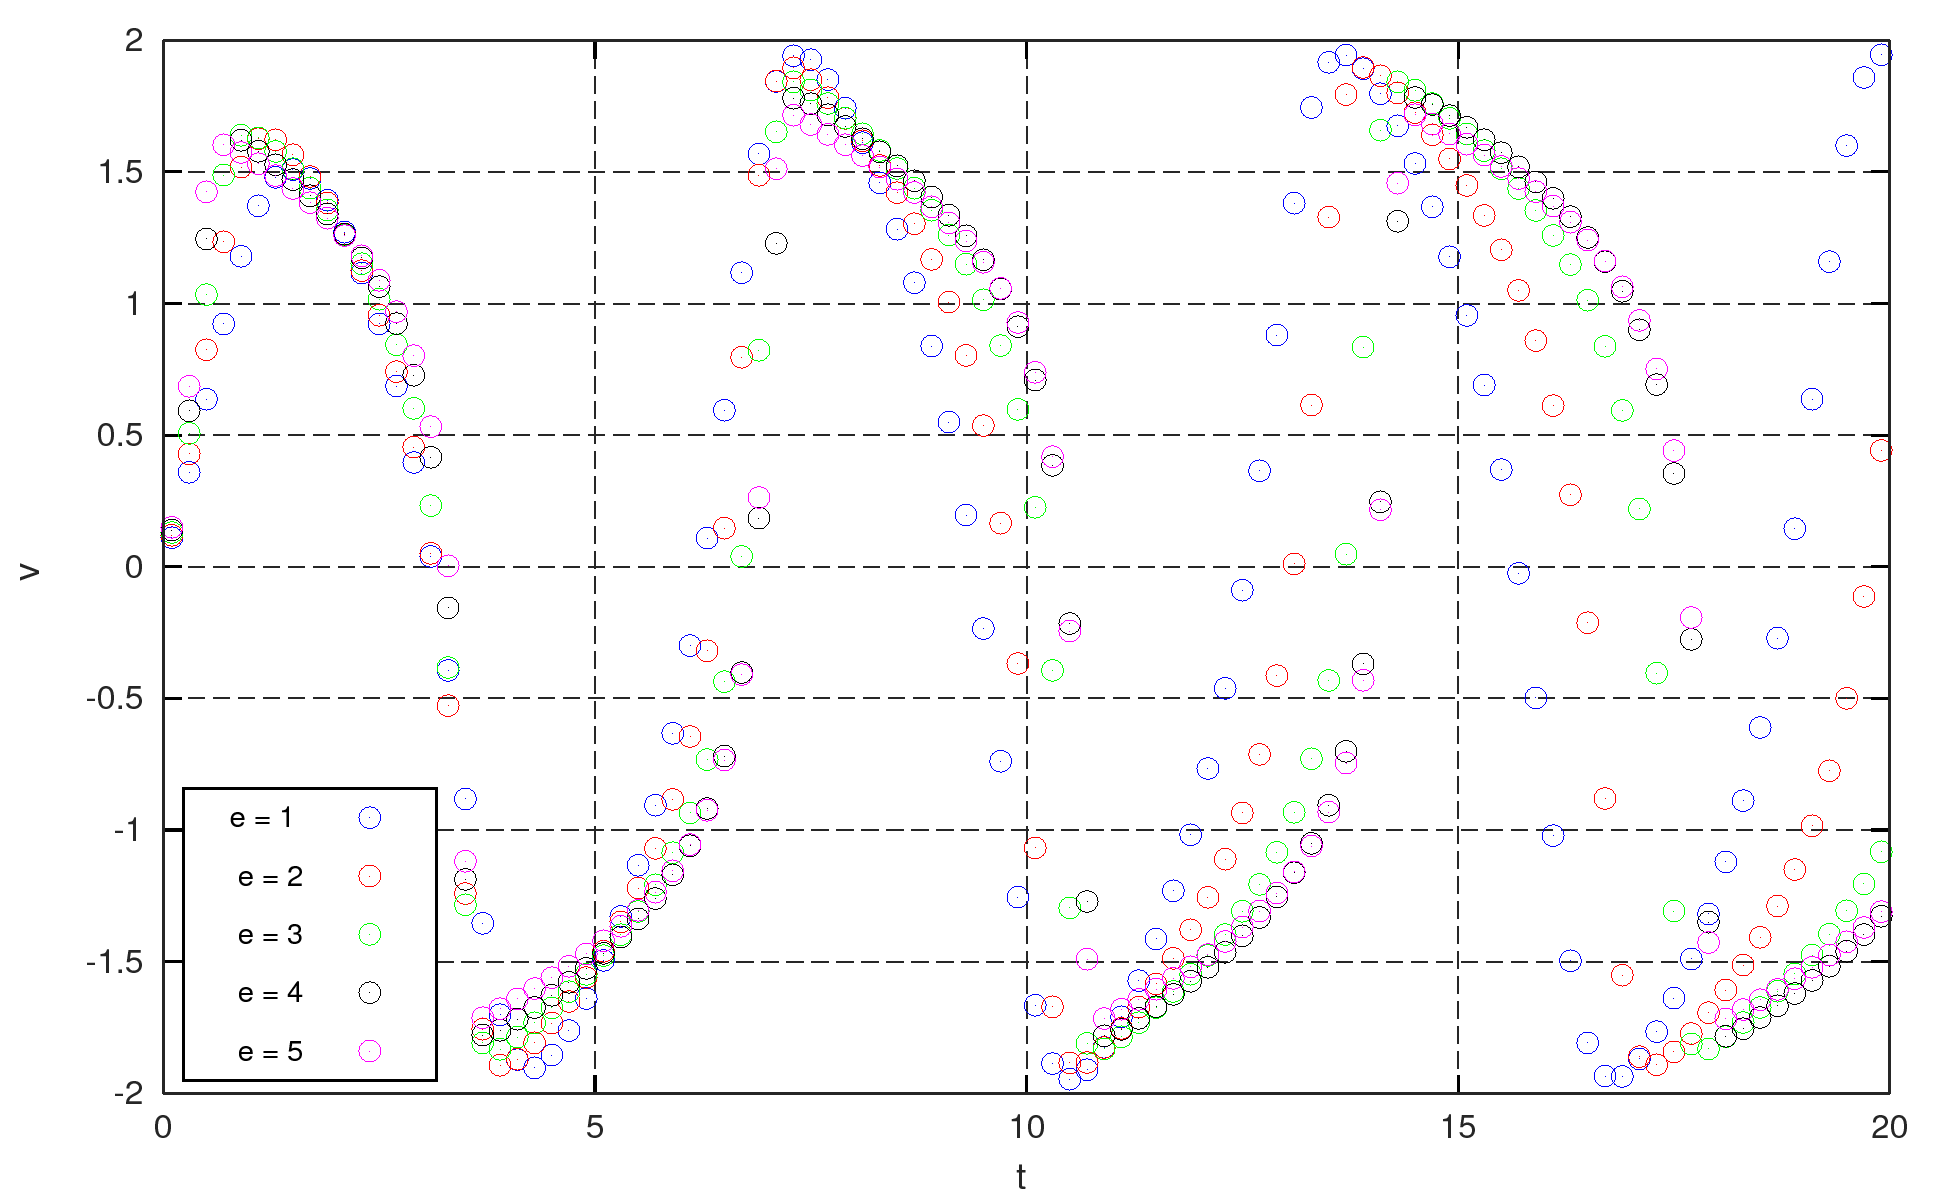
\includegraphics[scale = 0.8]{metodo_euler.png}
\caption{Aproximación por método de Euler - Oscilaciones}
\end{figure}

\begin{figure}[H]
\centering
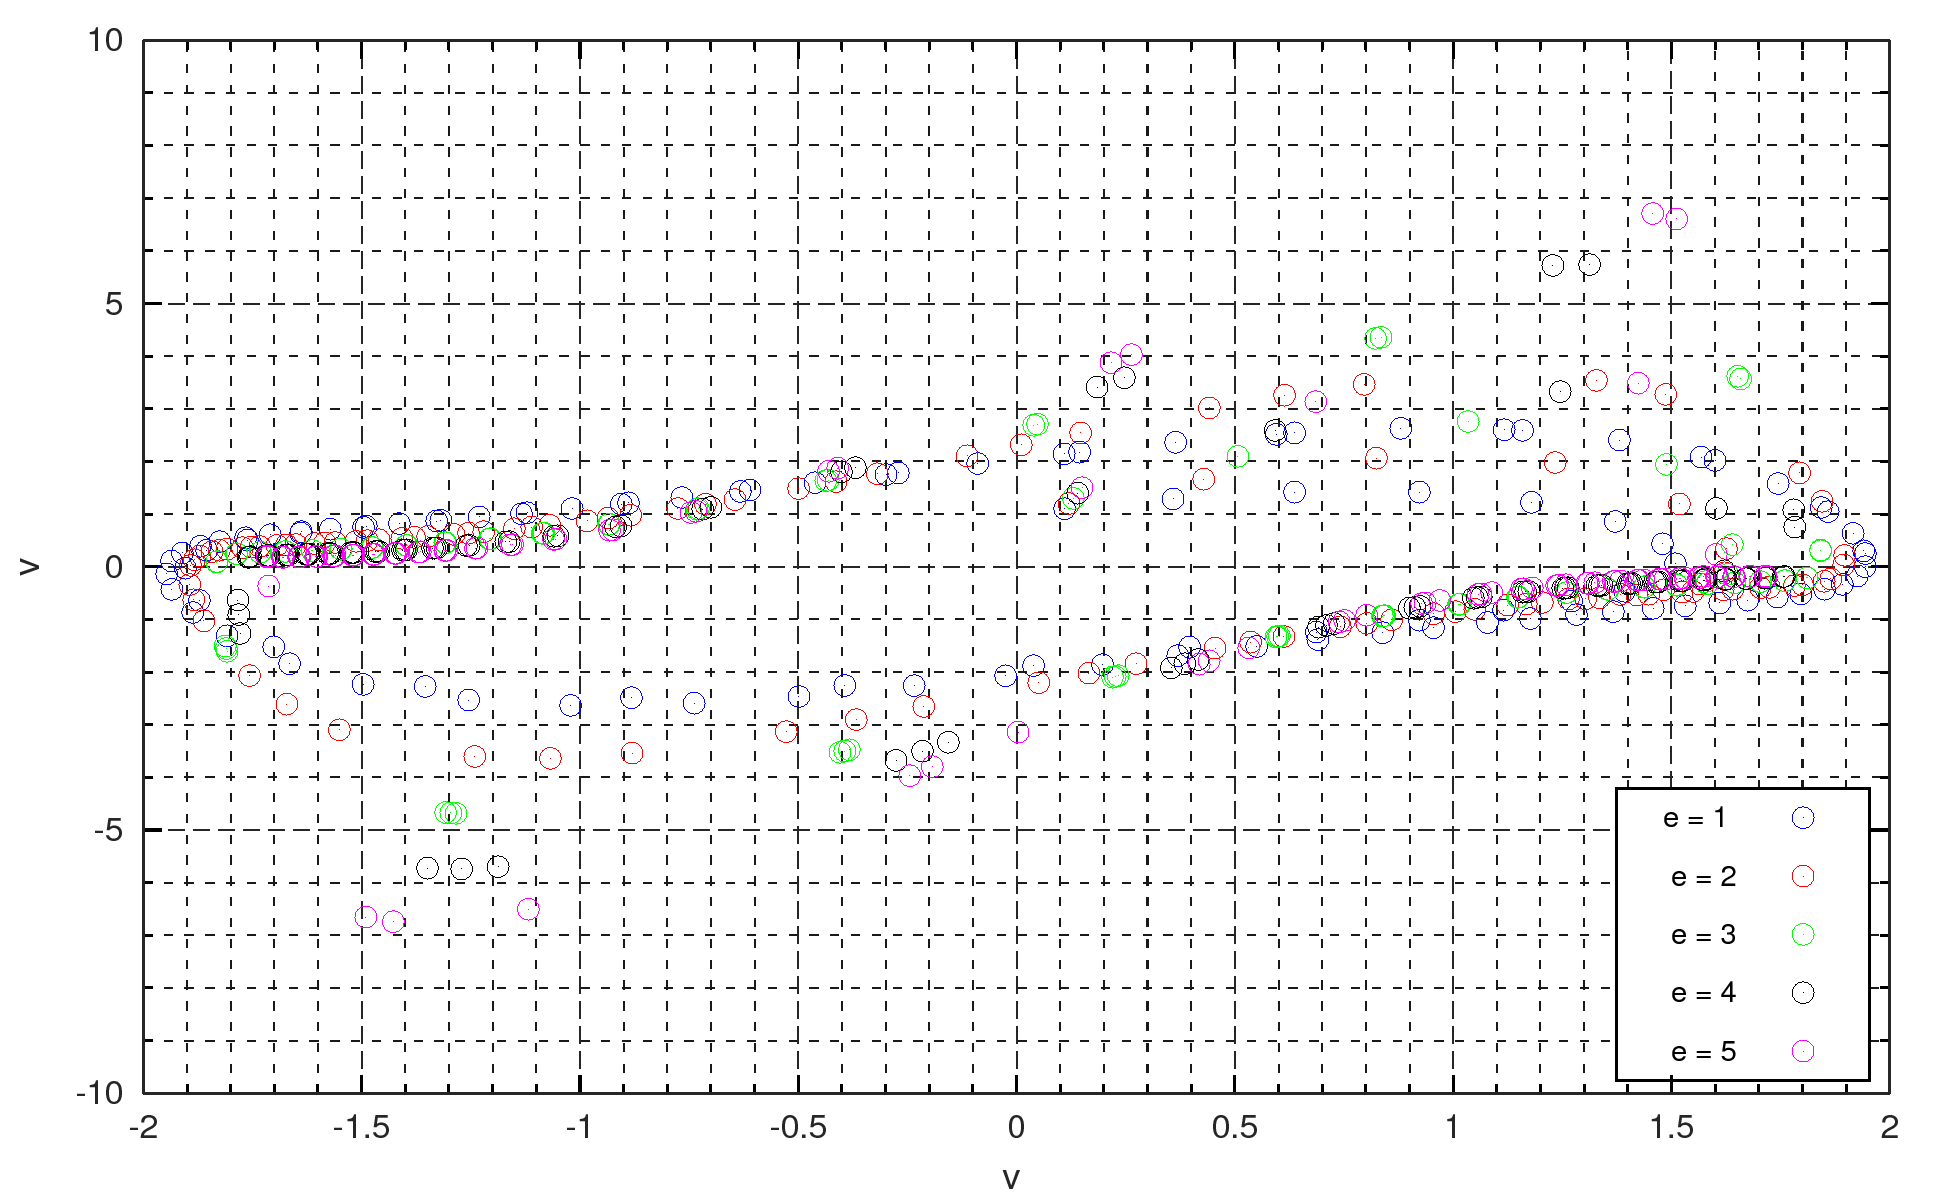
\includegraphics[scale = 0.8]{metodo_euler2.png}
\caption{Aproximación por método de Euler - Ciclos}
\end{figure}

\newpage
\subsection{Método de Runge-Kutta de segundo orden}
El método de Runge-Kutta es una generalización del del Euler para resolver ecuaciones diferenciales ordinarias de primer orden, pero en lugar de la una recta tangente se utiliza un promedio de varias pendientes de rectas en el intervalo $x_n < x <x_{n+1}$. El número de pendientes es el \textbf{orden} del método y a cada pendiente $k_i$ se le asigna un \textbf{peso} $w_i$. Los parámetros $w_i$ se eligen tal que la fórmula coincida con un polinomio de Taylor de grado m en  

\begin{equation}
y_{n+1} = y_n + h(w_1k_1 + ... + w_2k_m) 
\end{equation}

\begin{equation}
y(x_{n+1}) = y(x_n+h) = y(x_n) + hy'(x_n) + y''(x_n)\frac{h^2}{2!} +...+ y^{k+1}(c)\frac{h^{k+1}}{(k+1)!},\ \ x_n < c < x_{n+1} \nonumber
\end{equation}

En el caso del método con orden dos, hay que encontrar $w_1, w_2, \alpha, \beta$ tal que (YYYY) coincida con un polinomio de grado 2.Quedando determinados muchos posibles procedimientos de segundo orden.

\begin{equation}
y_{n+1} = y_n +h(w_1k_1 + w_2k_2) \nonumber
\end{equation}
\begin{equation}
k_1 = f(x_n,y_n),\ \ k_2= f(x_n+\alpha h, y_n + \beta k_1) \nonumber 
\end{equation}
\begin{equation}
w_1 = 1 - w_2,\ \ \alpha=\frac{1}{2w_2},\ \, \beta = \frac{1}{2w_2} \nonumber
\end{equation}

Tomando $w_2 = 1/2$ se tiene un porcedimento particular que ajustamos a nuestra nuestra ecuación de \textit{Van der Pol} mediante un cambio de variable $y = v'$
\begin{equation}
y_{n+1}  = y_n + \frac{h}{2}(k_1 + k_2)
\end{equation}
\begin{equation}
k_1 = \epsilon (1+v^2)y - v \nonumber
\end{equation}
\begin{equation}
v_{n+1} = v_n +\frac{h}{2}(2+h)y_n \nonumber
\end{equation}

\subsection{Simulación}
Tomando un h se discretiza un intervalo entre $[t_0, 3T]$, donde T representa un periodo de la oscilación de Van der Pol y $t_0$ un punto inicial. Tomando $t_0 = 0$ y $h=0.1$ se implementa un \textit{script} en \textit{Octave} para computar la aproximación numérica detallado en la figura TTTT.

\begin{center}
\begin{tabular}{c}
\\
\hline
\begin{lstlisting}
eps = [1:1:5] 	% Epsilon
h = 0.1		% Paso
n = 1 		% Contador

xn = 0 		% Condiciones
yn = 1
vn = 0

for n = [1:1:200]
	k1=eps.*(1-vn.^2).*yn - vn;
	k2 = eps.*(1-(vn+h).^2).*(yn+h.*k1) - (vn+h);
	yn1 = yn + (h/2).*(k1 + k2);
	
	yn = yn1;
	xn(n) = n*h;

	vn1 = vn + (h/2).*(2+h).*(yn);
	vn = vn1;
	n = n+1;
endfor
\end{lstlisting}
\\
\hline
\end{tabular}
\end{center}

\newpage

\begin{figure}[H]
\centering
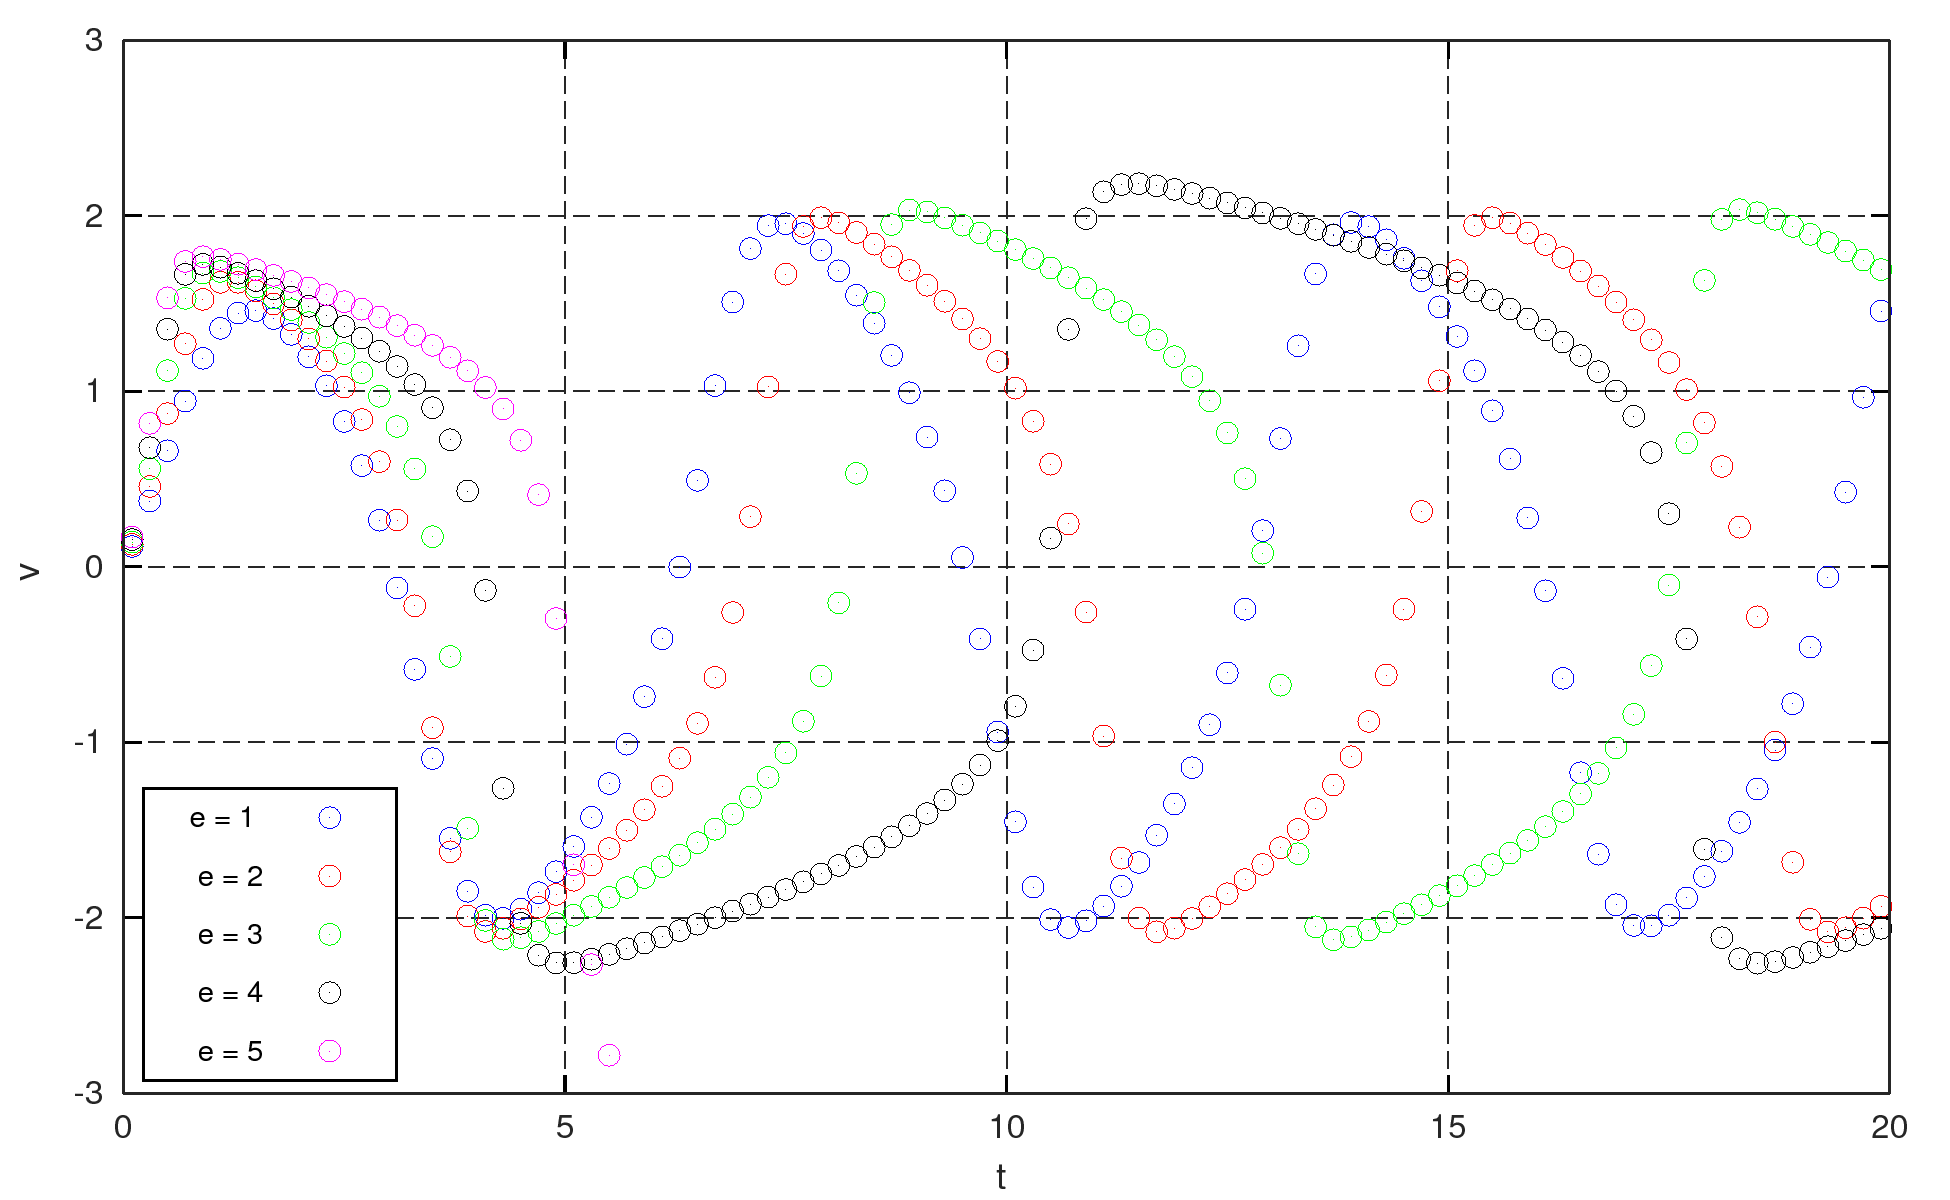
\includegraphics[scale = 0.8]{kr2a.png}
\caption{Aproximación por método de Rung-Kutta - Oscilaciones}
\end{figure}

\begin{figure}[H]
\centering
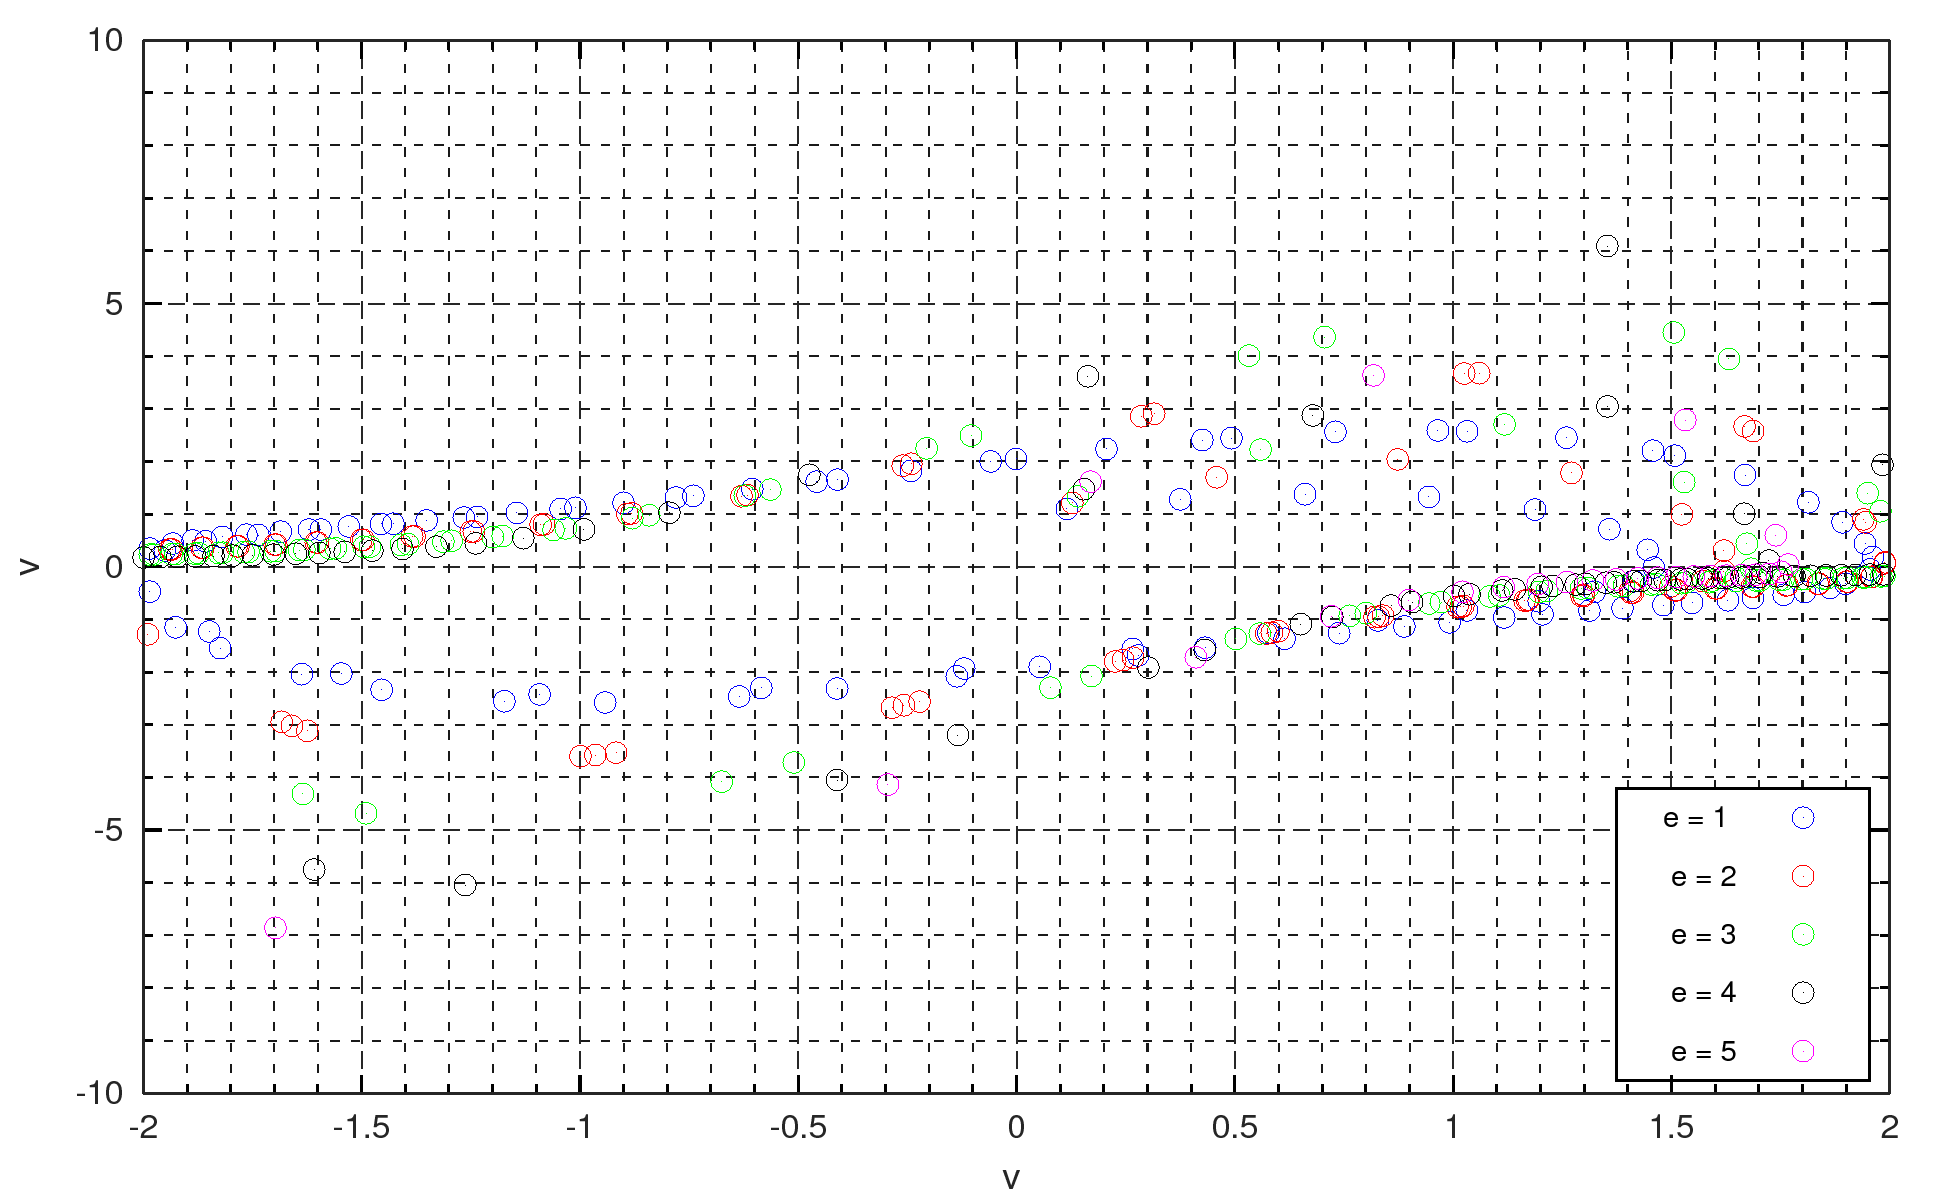
\includegraphics[scale = 0.8]{kr2b.png}
\caption{Aproximación por método de Runge-Kutta - Ciclos}
\end{figure}


\newpage
\section{Referencias}
\begin{enumerate}[{[}1{]}]
  \item Resumen de clases teóricas - Ing. Rodolfo Schwarz - 2011.
  \item Análisis numérico - Hernan González - 2da edición.
  \item Período Van der Pol \\\small\url{https://math.stackexchange.com/questions/1564464/how-to-find-the-period-of-periodic-solutions-of-the-van-der-pol-equation}
  \item \url{https://math.stackexchange.com/questions/1515251/using-rk4-on-the-van-der-pol-oscillator}
  \item Ecuación Diferenciales con aplicaciones de modelado - Dennis Zill - Cencage - Novena Edición - Capítulo 9.
\end{enumerate}






\end{document}